\chapter{Testování}\label{testovani}
% Nedílnou součástí vývoje softwaru je testování. Testování bylo rozděleno do dvou vrstev. Základní vrstvou jsou unit testy. Pro tvorbu těchto testů byl použit framework JUnit 5. Druhou vrstvou jsou integrační testy, které jsou implementovány pomoci funkcionality, kterou poskytuje framework Spring.
% Testování je nedílnou součástí implementace libovolného softwaru a je jeho velice důležitou častí. V rámci této bakalářské práce testům byla věnovaná řádná pozornost, proto bylo vyřešeno věnovat testům samostatnou kapitolu.
V teto kapitole bude popsán proces testování a doplňující funkcionalita, zjednodušující proces testování. Také bude popsáno pokrytí kódů testy.

\section{Tagy}\label{testovani:tagy}
    Tagy už byly zmíněné v sekci \ref{navrh:testovani}, ale jejích chování nebylo podrobně popsáno, proto je potřeba na začátku popsat chování tagů a proč je potřebujeme. Tagy označují jednotlivé testy nebo celé testovací třídy pomocí obyčejného textového řetězce (viz obrázek \ref{code:tag-junit-5}). Obsah řetězce může být libovolný. Za účelem pohodlnějšího využití tagů, byly zvolené řetězce, které popisuje konkretní aspekt chování testu. Například, pomalý test nebo integrační test. Při spouštěni testů pomocí frameworku JUnit můžeme definovat testy které bychom potřebovali spustit pomocí těchto předem definovaných tagů.
    
    Stejného výsledku bychom mohli dosáhnout pomocí třídění testů do různých složek, ale podstatný rozdíl mezi těmito postupy je v tom, že jeden test může mít několik tagů najednou a přidání nebo odstranění tagu je jednoduché . Například test může být anotován jako pomalý integrační test a zároveň jako pomalý test, kvůli tomu, že provádí databázovou transakci. Dosáhnout stejného výsledku pomocí třídění testu do specifických složek je náročnější a nedovoluje umístit test do několika složek najednou.
    \begin{figure}
        \begin{minted}{java}
@Tags(
        Tag("integration_test")
)
        \end{minted}
        \caption{Příklad tagu frameworku JUnit 5} 
        \label{code:tag-junit-5}
    \end{figure}
    
    Tagy jsou jenom textové řetězce, proto je docela očividně, že je velká pravděpodobnost překlepu při implementací velkého počtu testů\footnote{v době odevzdání bakalářské práci bylo implementováno 126 testů v 25 třídách}. Proto bylo vyřešeno definovat vlastní anotace s předem definovanými tagy. Ve výsledku byly implementovány 4 tagy:
    \begin{itemize}
            \item \verb|IntergationTest|, který má tag obsahující text \enquote{integration\_test}
            \item \verb|SecurityTest|, který má tag obsahující text \enquote{security\_test}
            \item \verb|SlowTest|, který má tag obsahující text \enquote{slow\_test}
            \item \verb|UnitTest|, který má tag obsahující text \enquote{unit\_test}
    \end{itemize}
    
    \begin{figure}
        \begin{minted}{java}
/**
 * Specifies test as a Integration test.
 */
@Target(allowedTargets = [
        AnnotationTarget.FUNCTION,
        AnnotationTarget.ANNOTATION_CLASS,
        AnnotationTarget.CLASS
])
@Retention(AnnotationRetention.RUNTIME)
@MustBeDocumented
@Tags(
        Tag("integration_test")
)
annotation class IntegrationTest
        \end{minted}
        \caption{Příklad třídy \texttt{Annotation} zaměňující tag s textem \enquote{integration\_test}} 
        \label{code:annotation-class}
    \end{figure}
    Anotace mají stejnou implementací a liší se jenom pomocí textu uvnitř tagů. Kotlin poskytuje funkcionalitu pro vytváření vlastních anotací, proto byla využita vestavěna třída anotace (viz obrázek \ref{code:annotation-class}). Anotace jsou implementovány takovým způsobem, že pomocí ně je možné anotovat ne jenom testové metody, ale i celé třídy. Pak anotace se aplikuje na každý test, který obsahuje anotovaná třída. Také je možné anotovat i jiné anotace.

    \begin{figure}
        \begin{minted}{groovy}
tasks.test {
    useJUnitPlatform()
    testLogging {
        events 'PASSED', 'FAILED', 'SKIPPED'
    }

    maxHeapSize = "1G"
}

task unitTests(type: Test) {
    useJUnitPlatform {
        includeTags 'unit_test'
    }
    testLogging {
        events 'PASSED', 'FAILED', 'SKIPPED'
    }
}

task integrationTests(type: Test) {
    useJUnitPlatform {
        includeTags 'integration_test'
    }
    testLogging {
        events 'PASSED', 'FAILED', 'SKIPPED'
    }
}
        \end{minted}
        \caption{Úkoly pro spouštění testů} 
        \label{code:gradle-tests}
    \end{figure}
    Pro spouštění testů je potřena využit nástroj pro automatizaci sestavování programu -- Gradle, který byl podrobně popsán v sekcí \ref{resere:build} . Testy jsou rozdělené podle jejich typu pomocí tagů, proto byla přidána možnost, nejenom spustit všechny testy najednou, ale i spustit jenom unit testy nebo jenom integrační testy (viz obrázek \ref{code:gradle-tests}). Kombinací tagů je mnohem více, ale konfigurační soubor obsahuje jenom konfigurace, které potřeboval autor teto práce během vývoje. Avšak přidat další konfigurace není složitě. Potřebujete jenom okopírovat předchozí konfigurací v konfiguračním souboru a změnit seznam tagů podle potřeby. Seznam tagů je také možné doplnit. Všechny aktuální tagy se nachází ve složce \verb|src/test/kotlin/cz/cvut/fit/sp/rozvody/annotation/tag| .
    
    Spuštění testů není omezené jenom příkazovou řádkou. Testy je také možné spustit pomocí vývojového prostředí nebo jiných nástrojů. Například, vývojové prostředí IntelliJ IDEA. 
    % Během vývoje velkých projektů zpouštění testů je významným problémem pro programátory. 
    % Framework JUnit 5 poskytuje možnost označovat metody a třídy pomocí tagu.
\section{Zobrazování testů}\label{testovani:zobrazovani}
    % TODO v pripade ze pobezi testy pres IDEA. Pres terminal nefunguje CamelCaseGenerator
    Správné a pochopitelné zobrazování názvů testu mnohem zjednodušuje proces testování. Proto před začátkem implementaci testů bylo navrženo pravidlo pro zobrazování testu. Název testu má obsahovat v stručný popis toho, co by měl test otestovat. 
    
    \begin{figure}\centering
	   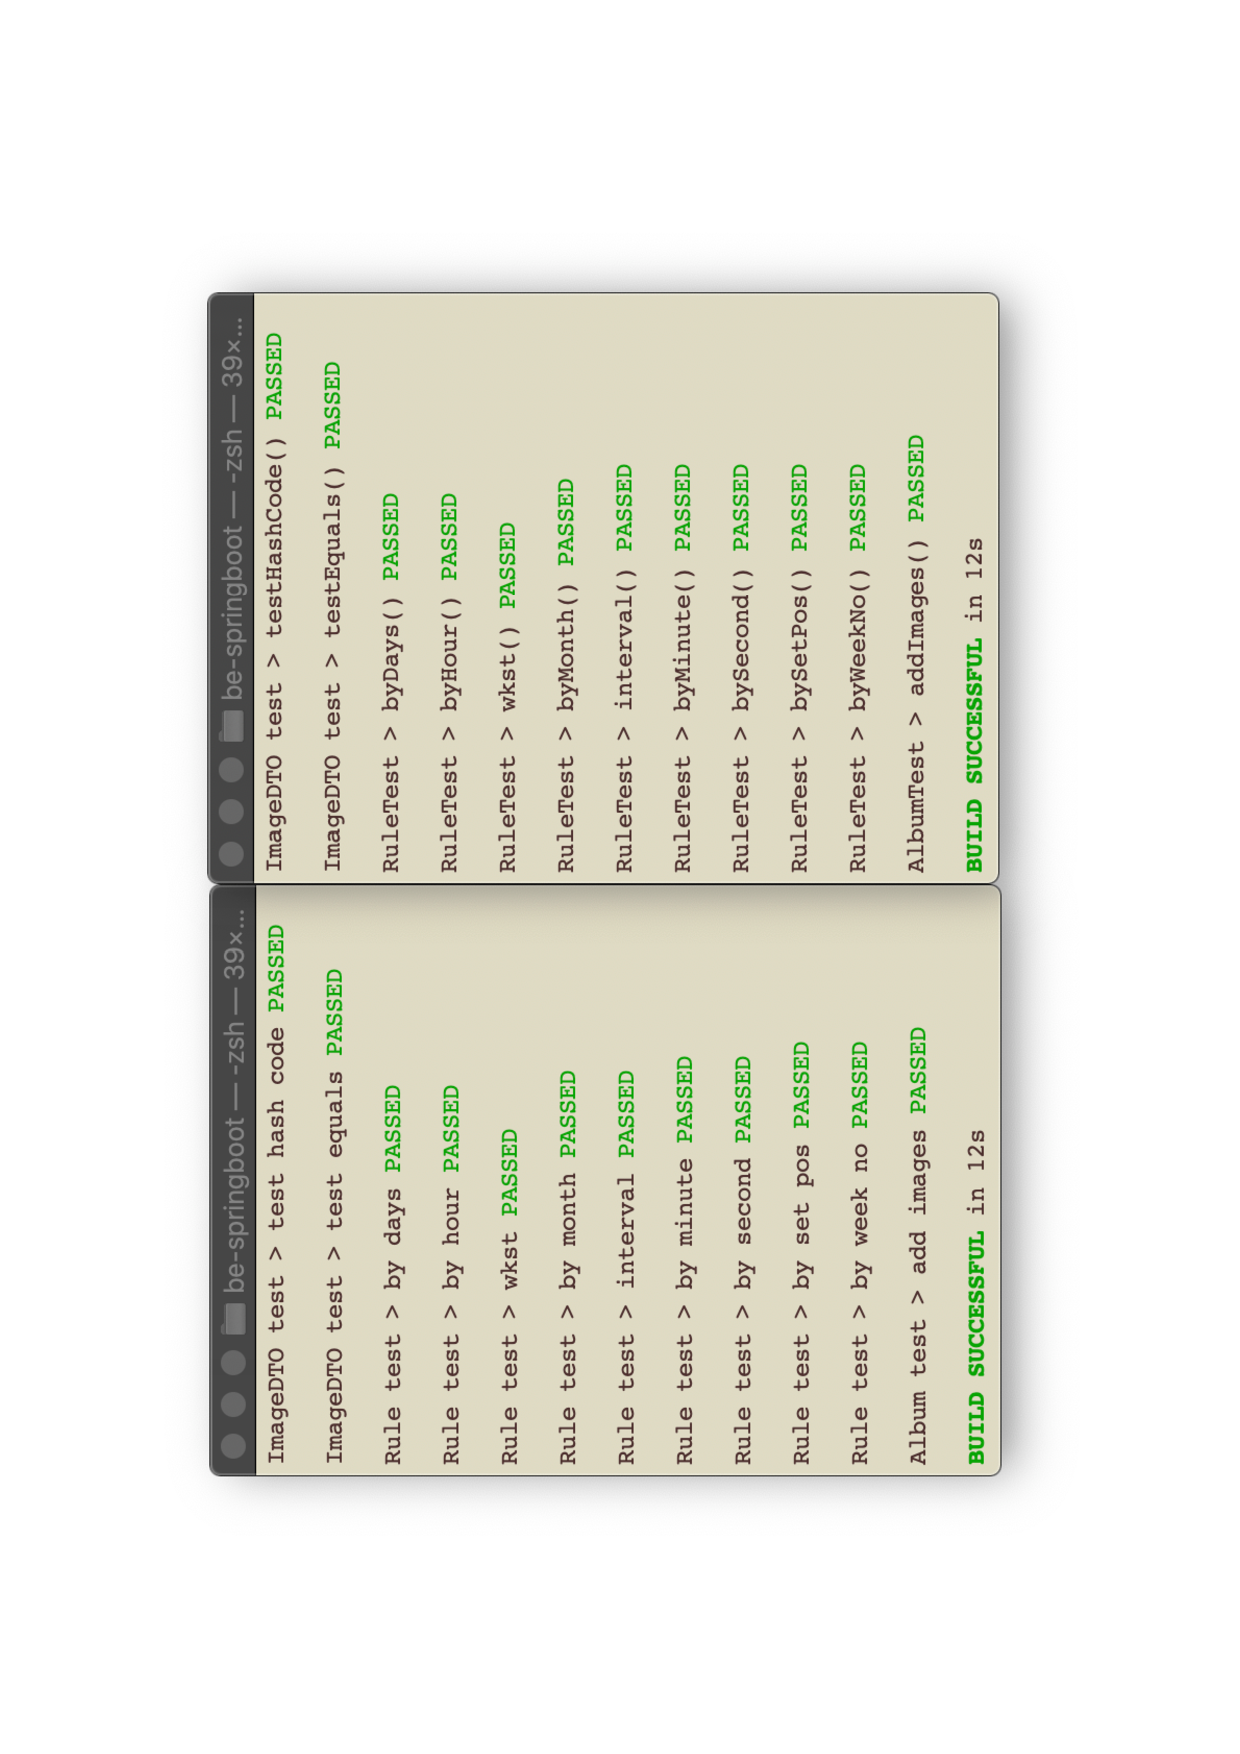
\includegraphics[angle=-90, width=1.0\textwidth]{pdfs/pretty-tests-comparison}
	   \caption[Srovnaní zobrazováni kódu]{Příklad vypisování testů pomocí generátoru a bez využití generátoru}\label{image:pretty-tests-comparison}
    \end{figure}
    Pro čitelnější zobrazování byl implementován generátor transformující jméno testu nebo jméno třídy do čitelnější podoby (viz obrázek \ref{image:pretty-tests-comparison}). Princip fingování je založen na překladu názvu z velbloudí notace na obyčejný text s mezerami. Výsledné názvy testů nebo tříd neobsahují žádné zbytečné symboly\footnote{například, za zbytečné symboly jsou považovány prázdné závorky na konci názvu metody}. Pro pohodlné využiti generátoru byla implementována anotace, která je aplikovatelná na třídy a metody. Anotace aktivuje generátor pro všechny testy, které třída obsahuje nebo pro konkretní test na který byla aplikována.
    
    V případě, že název metody obsahuje text, který by se neměl korektně transformovat, potřebujeme použit anotaci \verb|DisplayName| a v závorkách teto anotaci uvést text, který by měl být zobrazen. Tento název přepisuje výsledek generátoru, proto tato anotace může být použita ve třídě, která má anotaci generátoru. Příkladem takového nevhodného názvu může být třída se jménem \verb|ImageDTO|, která bude přeložena na \enquote{Image~d~t~o}, což zjevně není požadováným výsledkem.
    
\section{Unit testy}\label{testovani:unit}
    % Unit testy jsou zaměřené na otestování samostatně testovatelných metod a tříd
    Unit testy jsou zaměřené na otestování samostatně testovatelných metod a tříd. Všechny unit testy jsou anotovány jako unit testy (viz sekci \ref{testovani:tagy}) za účelem přidání možnosti spustit tyto testy zvlášť od ostatních testů. Žádný z testů není závislý na celém kontextu aplikace nebo její části, proto všechny unit testy jsou rychle.
    
\section{Integrační testy}\label{testovani:intergacni}
    % TODO Integrační testy zaměřené na ověření správné komunikace mezi komponentami aplikace.
    Velka pozornost byla věnovaná integračním testům. Tyto testy ověřují, jestli jednotlivé komponenty aplikace pracuje podle jejích návrhu. Testy jsou anotovány jako integrační testy (viz sekci \ref{testovani:tagy}) za účelem přidání možnosti spustit tyto testy zvlášť od ostatních, stejně jako unit testy. 
    
    Integrační testy vyžadují nahrání celého kontextu aplikace nebo jeho častí, proto jsou pomalejší než unit testy. Některé testy navíc mění kontext aplikace a vyžadují zničeni kontextu po dokončení jejich běhu. Takové test jsou anotovány jako pomalé testy\footnote{anotace \texttt{SlowTest}, obsahující tag \enquote{slow\_test}}.
    
        \begin{figure}
        \begin{minted}{java}
mvc.perform(
        MockMvcRequestBuilders
            .post("/api/v1/comment")
            .contentType(MediaType.APPLICATION_JSON)
            .content(commentDTO.toString())
)
    .andExpect(status().isCreated)
    .andExpect(content().contentType(MediaType.APPLICATION_JSON))
    .andExpect(jsonPath("$.createdById", is(
        commentDTO.createdById.toInt()
        )))
    .andExpect(jsonPath("$.text", is(commentDTO.text)))
    .andExpect(jsonPath("$.createdAt", is(
        commentDTO.createdAt.format(
            DateTimeFormatter.ISO_LOCAL_DATE_TIME
            )
        )))

        \end{minted}
        \caption{Příklad použití nástroje MockMvc} 
        \label{code:mockmvc}
    \end{figure}
    Většina integračních testů jsou zaměřená na ověření správného fungování vrstvy řadičů (\textit{controller}). Testování se provádí pomocí nástroje MockMvc\cite{mock-mvc}, který poskytuje framework Spring. Nástroj umožňuje otestovat funkcionalitu aplikace bez její úplného nastartování. Příklad využití nastroje je na obrázku \ref{code:mockmvc}. Tento kód má za úkol otestovat, zda řadič správně vytváří instanci entity \textit{Comment}. Kontrola správností atributu se provádí na základě DTO, který se vrátí jako návratová hodnota.
    
    V rámci integračních testu byly také ověřené přístupová práva (viz sekci \ref{navrh:bezpecnost}). Při testování řadičů bylo zapnuté filtrování podle role přihlášeného uživatele. Každému testu patří jeden uživatel, který je nastaven pomocí uživatelského jména\footnote{Uživatelským jménem v systému je adresa elektronické pošty}. V případě, že uživatel nemá dostatečná přístupová práva, řadič musí vrátit HTTP status s číslem 400\footnote{\textit{Bad Reques}t}.
    
\section{Samostatný profil pro testování}

    Testovaní aplikace vyžaduje vlastní nastavení, proto byl vytvořen samostatný profil, který odděluje testovací nastavení od nastavení produkce a vývoje. Profil má vlastní konfigurační soubor (\verb|application-test.properties|), obsahující nastavění databáze.
    
    Pro testování byla  využita stejná databáze jako i pro proces vývoje, za účelem kompletního a rychlého testování serveru. Databáze umožňuje rychle zničit a vytvořit tabulky, což nám umožňuje rychle zničit kontext aplikace mezi integračními testy.
    
    Také profil pro testování má vlastní implementaci pro \verb|UserDetailsService|\footnote{Základní rozhraní, které framework Spring využívá pro načítaní informace o uživateli}, obsahující tří implicitní uživatele:
    \begin{itemize}
            \item \verb|root|, vlastnící role \enquote{ROLE\_USER} a \enquote{ROLE\_ROOT} 
            \item \verb|userEmail|, vlastnící role \enquote{ROLE\_USER}
            \item \verb|user2Email|, vlastnící role \enquote{ROLE\_USER}
    \end{itemize}
    Tyto implicitní uživatel jsou využité v integračních testech pro spouštění požadavků (\verb|request|) přes instanci MocMvc. Podrobněji integrační testy byly popsány v sekci \ref{testovani:intergacni}.
    
\section{Pokrytí kódu testy}\label{testovani:pokryti}
    % TODO V teto sekci je uveden popis provedéní analýzy pokrýtí kódu testy.
    V teto sekci bude popsáno pokrytí kódů testy a uvedeny statistiky. Za účelem zvýšení přesnosti provedené analýzy, byly využité speciální nástroje pro zhodnocení pokrýti kódů.
    
    \subsection{JaCoCo}
    Prvním nástrojem, který byl využit pro analýzu testů, je Jacoco. Tento nástroj byl podrobně popsán v sekci \ref{resere:testovani:jacoco} . V teto sekci uvedeme jenom proces analýzy a její výsledky.
    
    JaCoCo vyžaduje implementování vlastního úkolu\footnote{Konfigurovatelný úkol pro nástroj Gradle. Například, \texttt{test} nebo \texttt{build}}(\verb|task|) v Gradle. Tento úkol byl nazván \verb|jacocoTestReport| a je možné ho spustit přes příkazovou řádku. Generování výsledků závisí na spouštění klasického úkolu \verb|test| od Gradle. 
    
    Generování výsledků pokrýti testů bylo využito jako nápověda pro identifikování důležitého kódu nepokrytého testy. Proto úkol \verb|jacocoTestReport| byl spouštěn několikrát. Podle poslední verze výsledku, která byla spouštěna pro poslední verzi aplikace, 85 \% instrukcí jsou pokryté testy. Podrobnou informaci se můžete dozvědět v příloze \ref{dodatek:code-coverage}.
    % vestaveny junit engine v IntelifIDEA prestal fingovat po dosazeni velkeho poctu testu
    \subsection{IntelliJ IDEA}
    Druhým testovacím nástrojem, který byl využit pro zjištění pokrytí kódů testy, je InteliJ~IDEA. Podrobněji tento nástroj byl popsán v sekci \ref{resere:testovani:intellij-idea} . 
    
    Tento nástroj také byl využit jako pomocný nástroj při implementaci testů. V teto sekci budou uvedený jenom výsledky posledního spouštění pro poslední verzi aplikace. Kompletní informaci o výsledcích najdete v příloze \ref{dodatek:code-coverage}.
    
    IntelliJ IDEA poskytuje trochu jinou informaci o pokrytí kódů než nástroj JaCoCo. Podle výsledku jsou pokryté testy:
    \begin{itemize}
            \item 72,6 \% tříd
            \item 90,1 \% metod
            \item 89,3 \% řádek kódů
    \end{itemize}